\documentclass[10pt]{exam}
\firstpageheader{Math 4050}{Worksheet \#10}{Name: Sunny Lee}
\usepackage{amsfonts}
\usepackage{amsmath}
\usepackage{amssymb, graphicx, enumerate, mathrsfs}

\begin{document}

\begin{enumerate}
    \item Since we do not apply the activation function for our input vector, we can 
    make a matrix of our weights and biases for the first layer: \\
    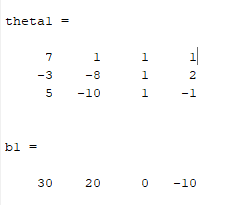
\includegraphics{theta1.png}\\
    Multiplying the input vector and the weights and adding the biases: \\
    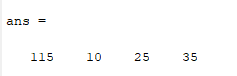
\includegraphics{a.png}\\
    Since none of these numbers are negative, this will be the vector which is passed 
    into the weights and biases of our output layer: \\
    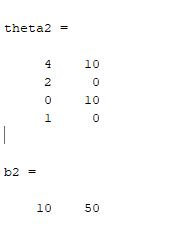
\includegraphics{b.png}\\
    Multiplying our input with these weights and adding the biases: \\
    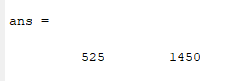
\includegraphics{c.png}\\
    Thus, the output for our neural network with an input of
     $x = \left[ 25, 10, -5 \right]$ is $\left[ 525, 1450 \right]$ since none of the
     ouputs are negative. 

\end{enumerate}


\end{document}